

\subsection{Sample Size Determination and Evaluation}

In the last chapter, two approaches used to determine the appropriate
sample size in the fixed-time step Monte Carlo simulations have been
proposed. One of them is based on inferential statistics
\cite{casella2002statistical}, which infers and estimates the unknown
population parameters from the sample statistics. Another one is
simpler since it does not need any simulations.

\subsubsection{Chebyshev's inequality}

According to LLN \cite{dekking2005modern}, the unknown population mean
first-passage time $\bar X$ can be estimated by sample mean $\bar X_N$
when $N$ is big enough. Chebyshev’s inequality
\cite{chebyshev1867valeurs} is a probabilistic inequality that can be
applied to any probability distribution of a random variable with the
finite expected value and non-zero variance. This inequality provides
an upper bound to the probability that the absolute deviation of a
random variable from its mean will exceed a given threshold.

\begin{figure}
  \begin{subfigure}{0.9\textwidth}
    \centering
    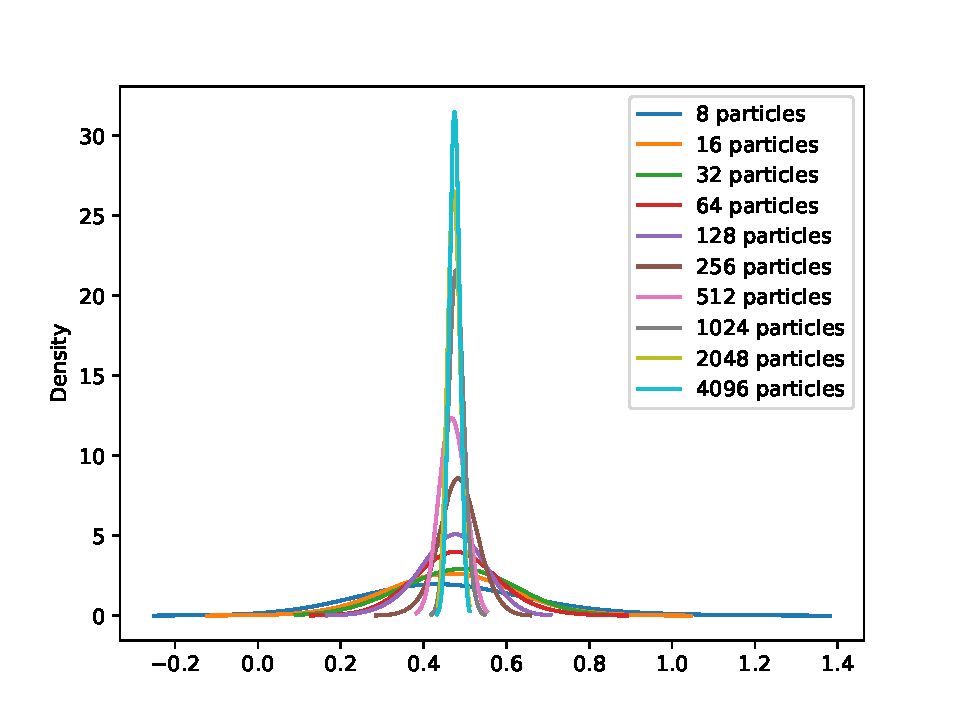
\includegraphics[width=0.9\textwidth]{kde}
    \caption{Running the LRWs in the annulus with $N = 2^i$
      particles and calculating the mean first-passage time $X_N$, where
      $i=3, 4, 5, ..., 12$. For each $N$, replicating the simulation
      $50$ times and recalculating the mean of the mean first-passage
      time $\bar X_{N}$ and the variance $\sigma^2_{N}$. As the sample
      size $N$ increase, the distribution of the sample means $X_N$
      becomes narrower and approximately normal. \label{fig:annulus_kde}}
  \end{subfigure}
  \begin{subfigure}{0.9\textwidth}
    \centering
    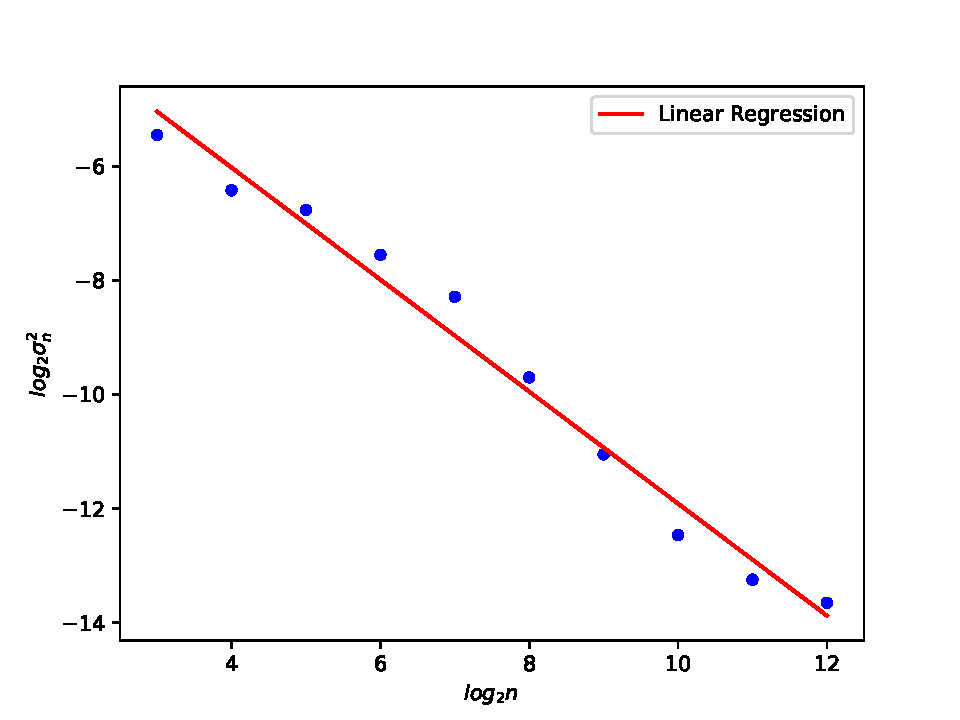
\includegraphics[width=0.8\textwidth]{linear_regression}
    \caption{A fitted linear regression model is used to explore the
      scaling relationship between $log_{2} (\sigma^2_{N})$ and
      $log_{2} N$. $log_{2} (\sigma^2_{N}) \approx b + k log_{2} N$,
      where $k$ and $b$ are the estimated model parameters, slope and
      intercept, respectively.\label{fig:annulus_linear_regression}}
  \end{subfigure}
  \caption{\label{fig:annulus_cheb}}
\end{figure}


In the Figure~\ref{fig:annulus_cheb}, the number of steps $t$ in the
numerical simulations have been converted into the unitless time
$\tau$ by the \highlight[id=Yuge, comment={No hard
    number}]{Eq.$(2.16)$}. Thus, given a predesignated error
$\epsilon$, the required number of particles $N$ can be determined by

\begin{equation}\label{eq:chab_substitute}
  Pr(|X_{N} - \bar X| \geq \epsilon) = Pr(|X_{N} - \bar X_{N}| \geq
  \epsilon) \leq \frac{\sigma^2_{N}}{\epsilon^2} \approx \frac{2^b
    N^k}{\epsilon^2} = 0.01
\end{equation}

where $\epsilon = 0.01 \bar X$.

The required number of particles in LRWs and PRWs can be estimated by
Eq.~\ref{eq:chab_substitute}, which is

\begin{equation}\label{eq:cheb_sample_size}
  N \geq (\frac{0.01 \epsilon^2}{2^b})^{\frac{1}{k}} \approx 1338643
\end{equation}

where $\epsilon \approx 0.004744$, $b \approx -2.088495$, and $k
\approx -0.982400$. Therefore, the number of particles should be at
least $1338643$ to make sure that there is no more than $1\%$ chance
of $X_N$ to be outside $[0.46865856, 0.47812641]$.


\begin{figure}
  \begin{subfigure}{0.9\textwidth}
    \centering
    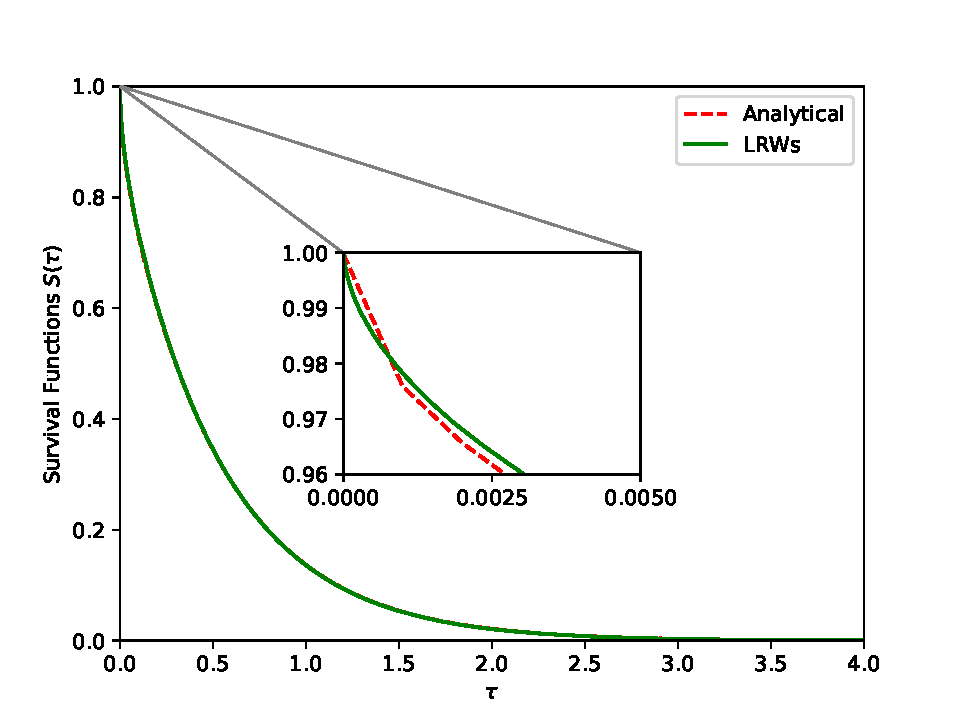
\includegraphics[width=0.8\textwidth]{LRWscheb}
    \caption{Survival curve for LRWs.\label{fig:LRW_survival}}
  \end{subfigure}
  \begin{subfigure}{0.9\textwidth}
    \centering
    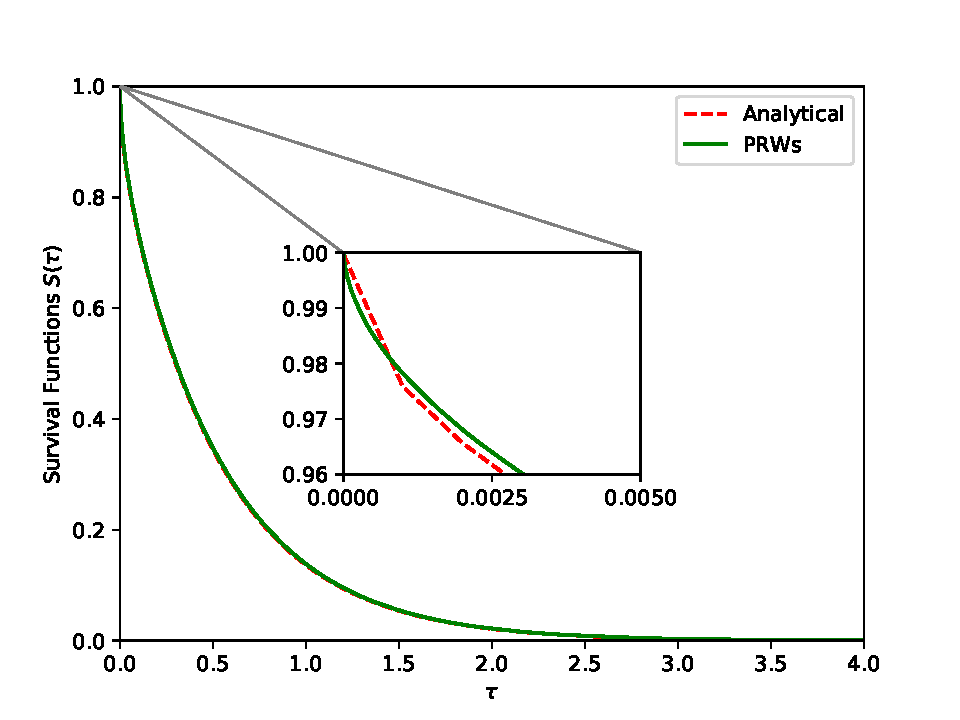
\includegraphics[width=0.8\textwidth]{PRWscheb}
    \caption{Survival curve for PRWs.\label{fig:PRW_survival}}
  \end{subfigure}
  \caption{Running PRWs and LRWs in the annulus with $1338643$
    particles determined by the Eq.~\ref{eq:cheb_sample_size} illustrating
    that the short and long time asypototic behaviors of the estimated
    survival functions of particles undergoing LRWs and PRWs are
    consistent with the analytical result in \highlight[{id=Yuge}]{Eq}}
  \label{fig:convergence_test}
\end{figure}

\begin{table}
  \centering
  \begin{tabular}{|c|c|c|}\hline
    Test Methods (standard nonparametric) & Statistics & P Values \\
    \hline
    Logrank & 0.017679 & 0.894223 \\
    \hline
    Fleming-Harrington & 0.742536 & 0.388850 \\
    \hline
    Gehan-Breslow & 0.742536 & 0.388850 \\
    \hline
    Tarone-Ware & 0.499418 & 0.479756 \\
    \hline
  \end{tabular}
  \caption{The estimated survival function of $1338643$ particles in
    the LRWs is statistically similar to the analytical survival
    function.}
  \label{tab:two_sample_test_lrws_analytical}
\end{table}

\begin{table}
  \centering
  \begin{tabular}{|c|c|c|}\hline
    Test Methods (standard nonparametric) & Statistics & P Values \\
    \hline
    Logrank & 0.039142 & 0.843168 \\
    \hline
    Fleming-Harrington & 0.083388 & 0.772757 \\
    \hline
    Gehan-Breslow & 0.083388 & 0.772757 \\
    \hline
    Tarone-Ware & 0.010582 & 0.918069 \\
    \hline
  \end{tabular}
  \caption{The estimated survival function of PRWs, which has
    $1338643$ particles with step length $0.5$, is not statistically
    different from the analytical survival function.}
  \label{tab:two_sample_test_prws_analytical}
\end{table}

From the visualized comparison in Figure~\ref{fig:convergence_test}
and the results of the two-sample statistical tests in
Table~\ref{tab:two_sample_test_lrws_analytical} and
Table~\ref{tab:two_sample_test_prws_analytical}, the fixed-step Monte
Carlo simulations' results converge to the analytical
outcomes. Therefore, the integral of the solutions of heat equations
can be approximated by the Monte Carlo simulations without calculating
manually. As mentioned in the last chapter, the integral, $S(\tau)$,
indicates the annulus' geometrical information. Therefore, the
fixed-time step Monte Carlo simulation can describe the shape of an
object without using the rulers. However, the number of particles in
the numerical simulations estimated by Eq.~\ref{eq:chab_substitute} is
abundant, which causes a high computational cost because each random
trajectories of each particle are simulated in LRWs and PRWs till they
reach the inner boundary of the annulus.


\subsubsection{Dvoretzky–Kiefer–Wolfowitz (DKW) inequality}

Chebyshev's inequality can be applied to any probability distribution,
but it is also weaker than other inequalities. DKW inequality is more
efficient since the confidence band is generated without running any
simulations. For example, let $F(\tau)$ be the true cumulative
distribution function (CDF) of the first passage time, a continuous unitless
random variable on the interval $[0, \infty]$. $F(\tau)$ has a
relationship with $S(\tau)$, which is

\begin{equation}\label{eq:cdf}
  F(\tau) = 1 - S(\tau)
\end{equation}

The true CDF is known by Eq.~\ref{eq:cdf}, which can also be approximated
numerically. A simple example of generating the CDF-based confidence
bounds by DKW inequality is shown in Figure~\ref{fig:dkw_cb_sample}. The empirical
distribution function $F_{256}(\tau)$ is estimated by the lifeline
module in Python \cite{davidson2019lifelines}. Thus, the interval
$\varepsilon$ contains the entire $F(\tau)$ with the probability
$95\%$ can be calculated by \highlight[id=Yuge]{Eq.$(2.20)$}

\begin{equation}\label{eq:dkw_cb}
  \varepsilon = \sqrt{\frac{\ln{\frac{2}{0.05}}}{2* 256}} \approx 0.084881
\end{equation}

\begin{figure}
  \centering
  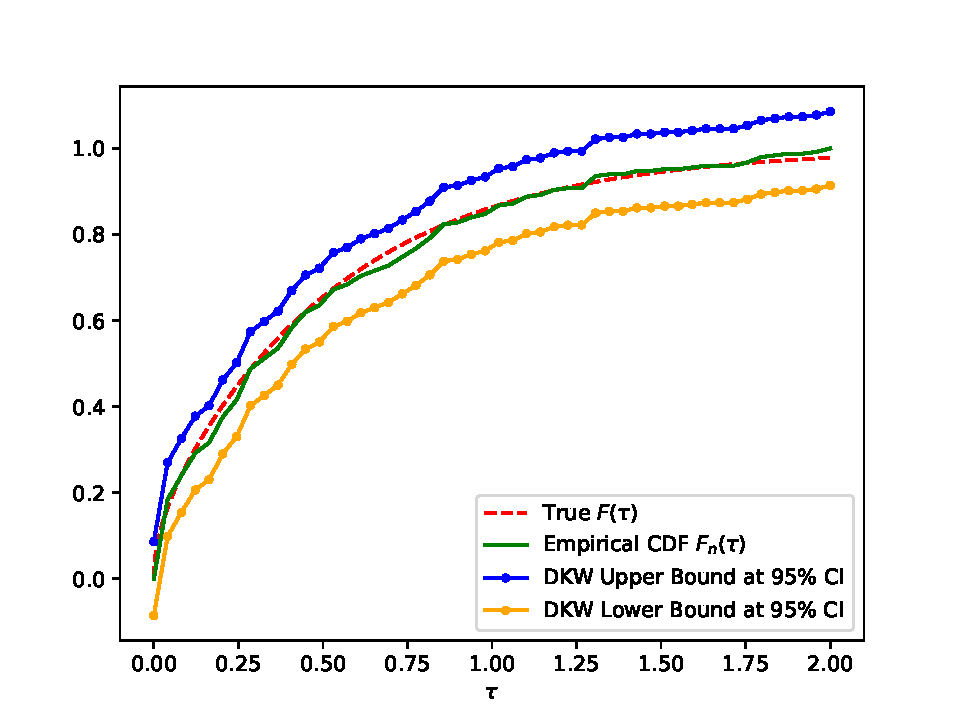
\includegraphics[width=0.8\textwidth]{dkw_comfidence_band_demo}
  \caption{The simultaneous band around $F_{256}(\tau)$ with interval
    $0.084881$ calculate by Eq.~\ref{eq:dkw_cb} encompasses
    the entire $F(x)$ at $95\%$ confidence level. \label{fig:dkw_cb_sample}}
\end{figure}



Moreover, the sample size estimated by DKW inequality \highlight[id=Yuge]{Eq.$(2.20)$} does
not depend on the geometries or the kind of simulations because the
simultaneous confidence bounds always contain the true cumulative
distribution at a specific confidence level. For instance, assume the
probability, that the maximum distance between $F_N(\tau)$ and
$F(\tau)$ is bigger than $0.005$, is smaller than $0.01$, the minimum
required number of particles should meet the inequality

\begin{equation}\label{eq:dkw_substitute}
  Pr(\sup_{x \in \mathbb{R}} |F_{N}(\tau) - F(\tau)| > 0.005) \leq 2e^{-2N0.005^2} = 0.01
\end{equation}

Thus, after the transformation of Eq.~\ref{eq:dkw_substitute}, the
sample size can be determined by

\begin{equation}\label{eq:dkw_sample_size}
  N \geq \frac{\ln(\frac{0.01}{2})}{-2 \times 0.005^2} \approx
  105966
\end{equation}


\begin{figure}
  \begin{subfigure}{0.9\textwidth}
    \centering
    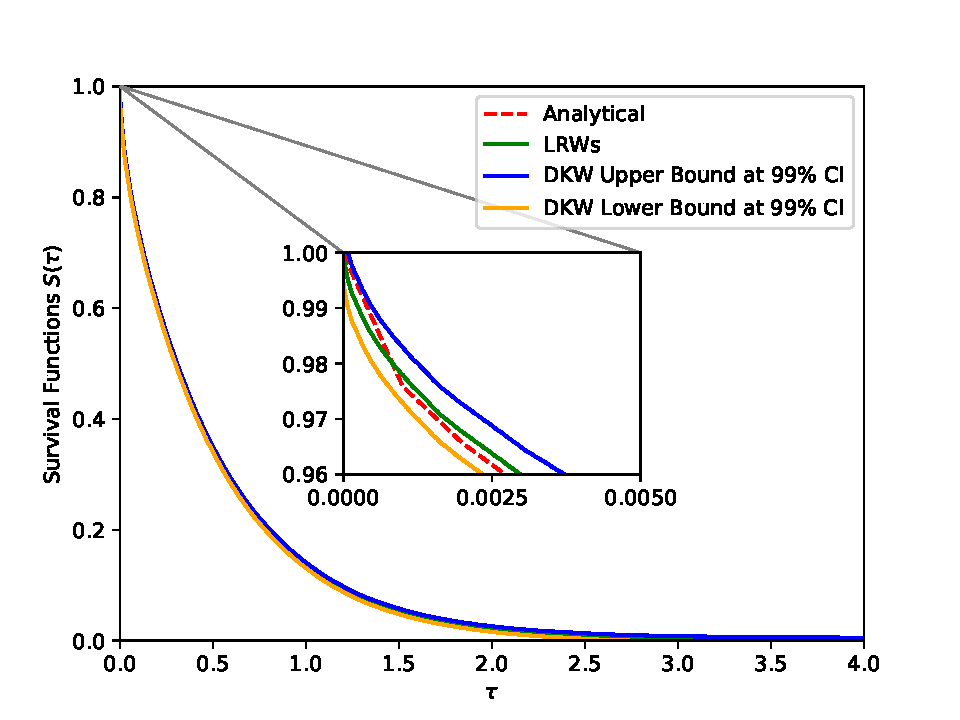
\includegraphics[width=0.8\textwidth]{LRWsdkw}
    \caption{The simultaneous confidence bands, generated by
      Eq.~\ref{eq:dkw_substitute}, of the estimated survival function
      $S(t)$ for LRWs contain the whole ture analytical
      $S(\tau)$. \label{fig:dkw_lrws_analytical}}
  \end{subfigure}
  \begin{subfigure}{0.9\textwidth}
    \centering
    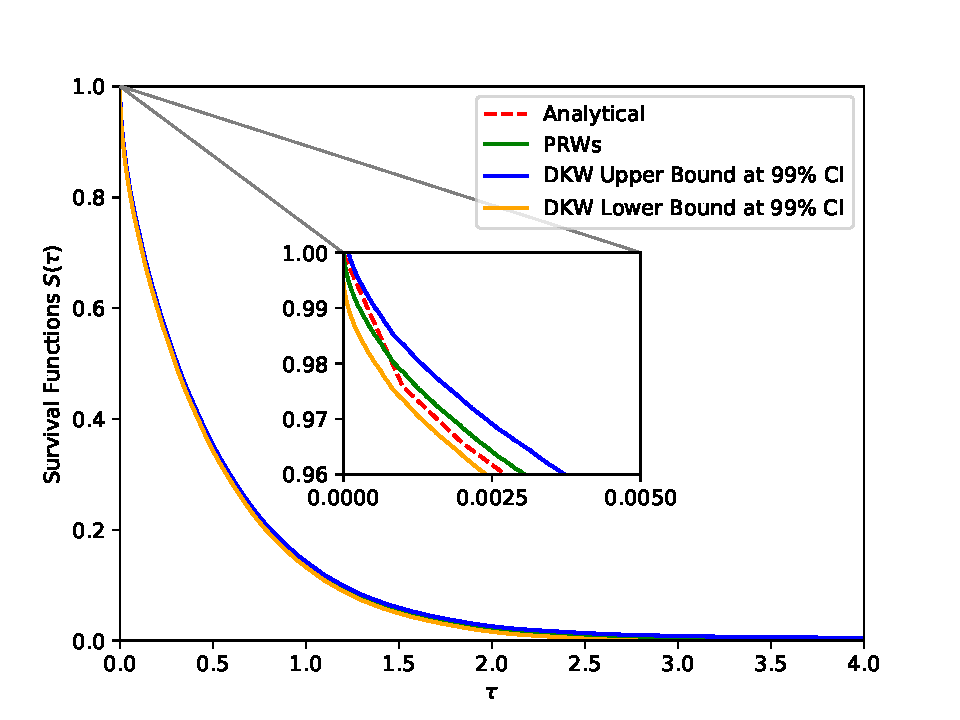
\includegraphics[width=0.8\textwidth]{PRWsdkw}
    \caption{The simultaneous confidence bands, generated by
      Eq.~\ref{eq:dkw_substitute}, of the estimated survival function
      $S(t)$ for PRWs contain the whole ture analytical
      $S(\tau)$. \label{fig:dkw_prws_analytical}}
  \end{subfigure}
  \caption{PRWs and LRWs are implemented in the annulus with $105966$
    particles determined by the Eq.~\ref{eq:dkw_sample_size}. (a) and
    (b) show that the DKW simultaneous confidence bands of estimated
    survival function with the interval $0.005$ encompass the entire
    analytical $S(\tau)$ at $99 \%$ confidence level. \label{fig:dkw_rw_analytical}}
\end{figure}

\begin{table}
  \centering
  \begin{tabular}{|c|c|c|}\hline
    Test Methods (standard nonparametric) & Statistics & P Values \\
    \hline
    Logrank & 1.532224 & 0.215779 \\
    \hline
    Fleming-Harrington & 1.630358 & 0.201654 \\
    \hline
    Gehan-Breslow & 1.630358 & 0.201654 \\
    \hline
    Tarone-Ware & 1.619530 & 0.203157 \\
    \hline
  \end{tabular}
  \caption{The estimated survival function of $105966$ particles in
    the LRWs is not statistically different to the analytical survival
    function.}
  \label{tab:two_sample_test_dkw_lrws_analytical}
\end{table}


\begin{table}
  \centering
  \begin{tabular}{|c|c|c|}\hline
    Test Methods (standard nonparametric) & Statistics & P Values \\
    \hline
    Logrank & 2.645624 & 0.103835 \\
    \hline
    Fleming-Harrington & 1.473674 & 0.224767 \\
    \hline
    Gehan-Breslow & 1.473674 & 0.224767 \\
    \hline
    Tarone-Ware & 1.986810 & 0.158675 \\
    \hline
  \end{tabular}
  \caption{The estimated survival function of PRWs, which has
    $105966$ particles with step length $0.5$, is statistically
    similar to the analytical survival function.}
  \label{tab:two_sample_test_dkw_prws_analytical}
\end{table}

From the Figure~\ref{fig:dkw_rw_analytical},
Table~\ref{tab:two_sample_test_dkw_lrws_analytical}, and
Table~\ref{tab:two_sample_test_dkw_prws_analytical}, although the sample
size in the LRWs and PRWs determined by DKW inequality is about $10$
times smaller than that by Chebyshev’s inequality, the estimated
survival functions of the numerical simulations converge to the
analytical results within the amount of statistical uncertainty.
